% Input common header
\documentclass[xcolor=dvipsnames]{beamer}

\usecolortheme[named=Blue]{structure}
\setbeamertemplate{itemize items}[circle]

\usepackage{smartdiagram}


\author{Dr. Paul Larsen}
\date{\today}

\usetikzlibrary{decorations}
\usetikzlibrary{snakes}

\title{Artificial Intelligence, Risk and Discrete Geometry}
\begin{document}
\maketitle

\begin{frame}{Risk, Regulation and Artificial Intelligence\footnote{What about discrete geometry? Just wait \ldots it shows up soon and keeps reappearing}}
  \framesubtitle{\ldots in one diagram}
  \begin{center}
    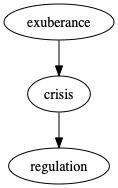
\includegraphics[width=0.3\textheight]{graphics/exuberance-crisis-regulation}
  \end{center}
\end{frame}

\begin{frame}{What is Risk Regulation?}
  \framesubtitle{A brief history of financial disaster}
  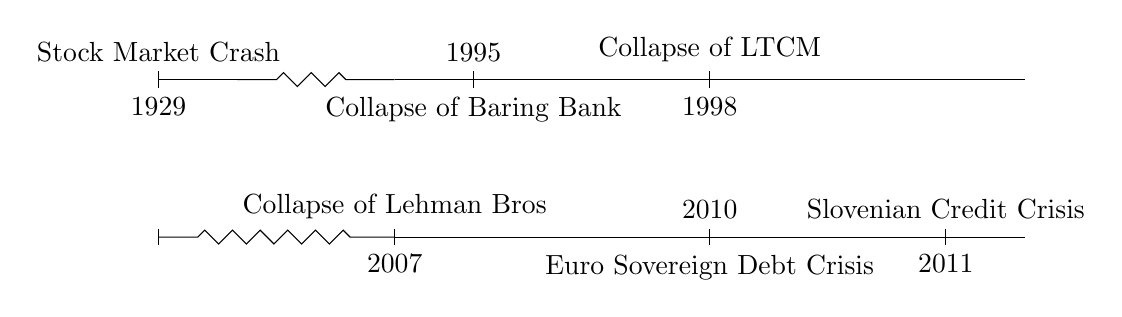
\begin{tikzpicture}[snake=zigzag, line before snake = 5mm, line after snake = 5mm]
    % draw horizontal line
    \draw (0,0) -- (1,0);
    \draw[snake] (1,0) -- (3,0);
    \draw (3,0) -- (11,0);
    % \draw[snake] (5,0) -- (7,0);

    % draw vertical lines
    \foreach \x in {0,4,7}
      \draw (\x cm,3pt) -- (\x cm,-3pt);

    % draw nodes
    \draw (0,0) node[below=3pt] {$ 1929 $} node[above=3pt] { Stock Market Crash };
    \draw (4,0) node[below=3pt] { Collapse of Baring Bank } node[above=3pt] {$ 1995 $};
    \draw (7,0) node[below=3pt] {$ 1998 $} node[above=3pt] { Collapse of LTCM };

    \draw[snake] (0,-2) -- (3,-2);
    \draw (3,-2) -- (11,-2);

    % draw vertical lines
    \foreach \x in {0,3,7,10}
      \draw (\x cm,-2.1) -- (\x cm,-1.9);

    % draw notes
    \draw (3,-2) node[below=3pt] {$ 2007 $} node[above=3pt] { Collapse of Lehman Bros };
    \draw (7,-2) node[below=3pt] { Euro Sovereign Debt Crisis } node[above=3pt] {$ 2010 $};
    \draw (10,-2) node[below=3pt] {$ 2011 $} node[above=3pt] { Slovenian Credit Crisis };
  %   \draw (6,0) node[below=3pt] {$  $} node[above=3pt] {$  $};
  %   \draw (7,0) node[below=3pt] {$ n $} node[above=3pt] {$ 10n $};
  \end{tikzpicture}
\end{frame}

\begin{frame}{What is Risk Regulation?}
  \framesubtitle{A cheeky guide to financial services risk types}
  \begin{block}{The risk of losing money due to \ldots}
    \begin{itemize}
      \item Credit: counter-party default
      \item Market: market movements
      \item Operational: something going wrong that shouldn't
      \item Liquidity: funding mismatches
      \item Insurance: unexpected loss of premiums or increase of claims
    \end{itemize}
  \end{block}

  \begin{block}{\ldots and the regulation that results from disasters big and small}
    \href{https://www.bis.org/basel_framework/}{Basil Framework (banking)},
    \href{https://www.eiopa.europa.eu/browse/solvency-2_en}{Solvency II (insurance)},
    \href{https://eur-lex.europa.eu/legal-content/EN/TXT/PDF/?uri=CELEX\%3A52021PC0206}{The AI Act (EU)},
    \href{https://www.bafin.de/SharedDocs/Veroeffentlichungen/EN/Meldung/2020/meldung\_2020\_05\_25\_KAIT\_en.html}{IT Requirements for German Asset Managers}
  \end{block}
\end{frame}


\begin{frame}{What is AI?}
\framesubtitle{Humans are amazing at navigating a world that does not make sense}
  \begin{tikzpicture}

    \node[inner sep=0pt] (grass) {
      \fbox{
          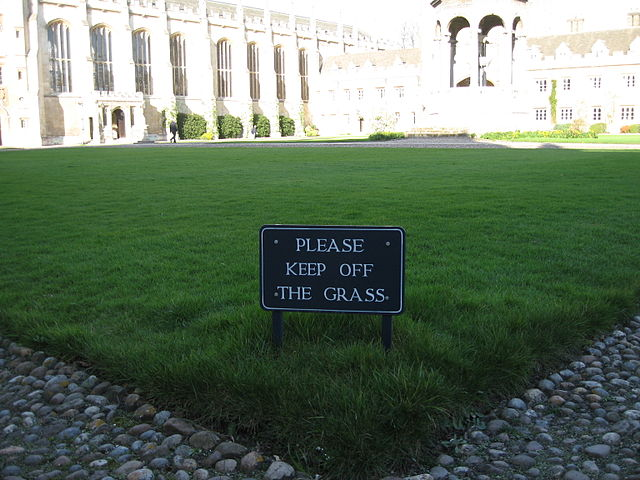
\includegraphics[width=0.7\textheight]{graphics/640px-Please_keep_off_the_grass_Great_Court_Trinity_College_Cambridge}
      }
    };
    \node[inner sep=0pt, right=0.5cm of grass] (door)  {
      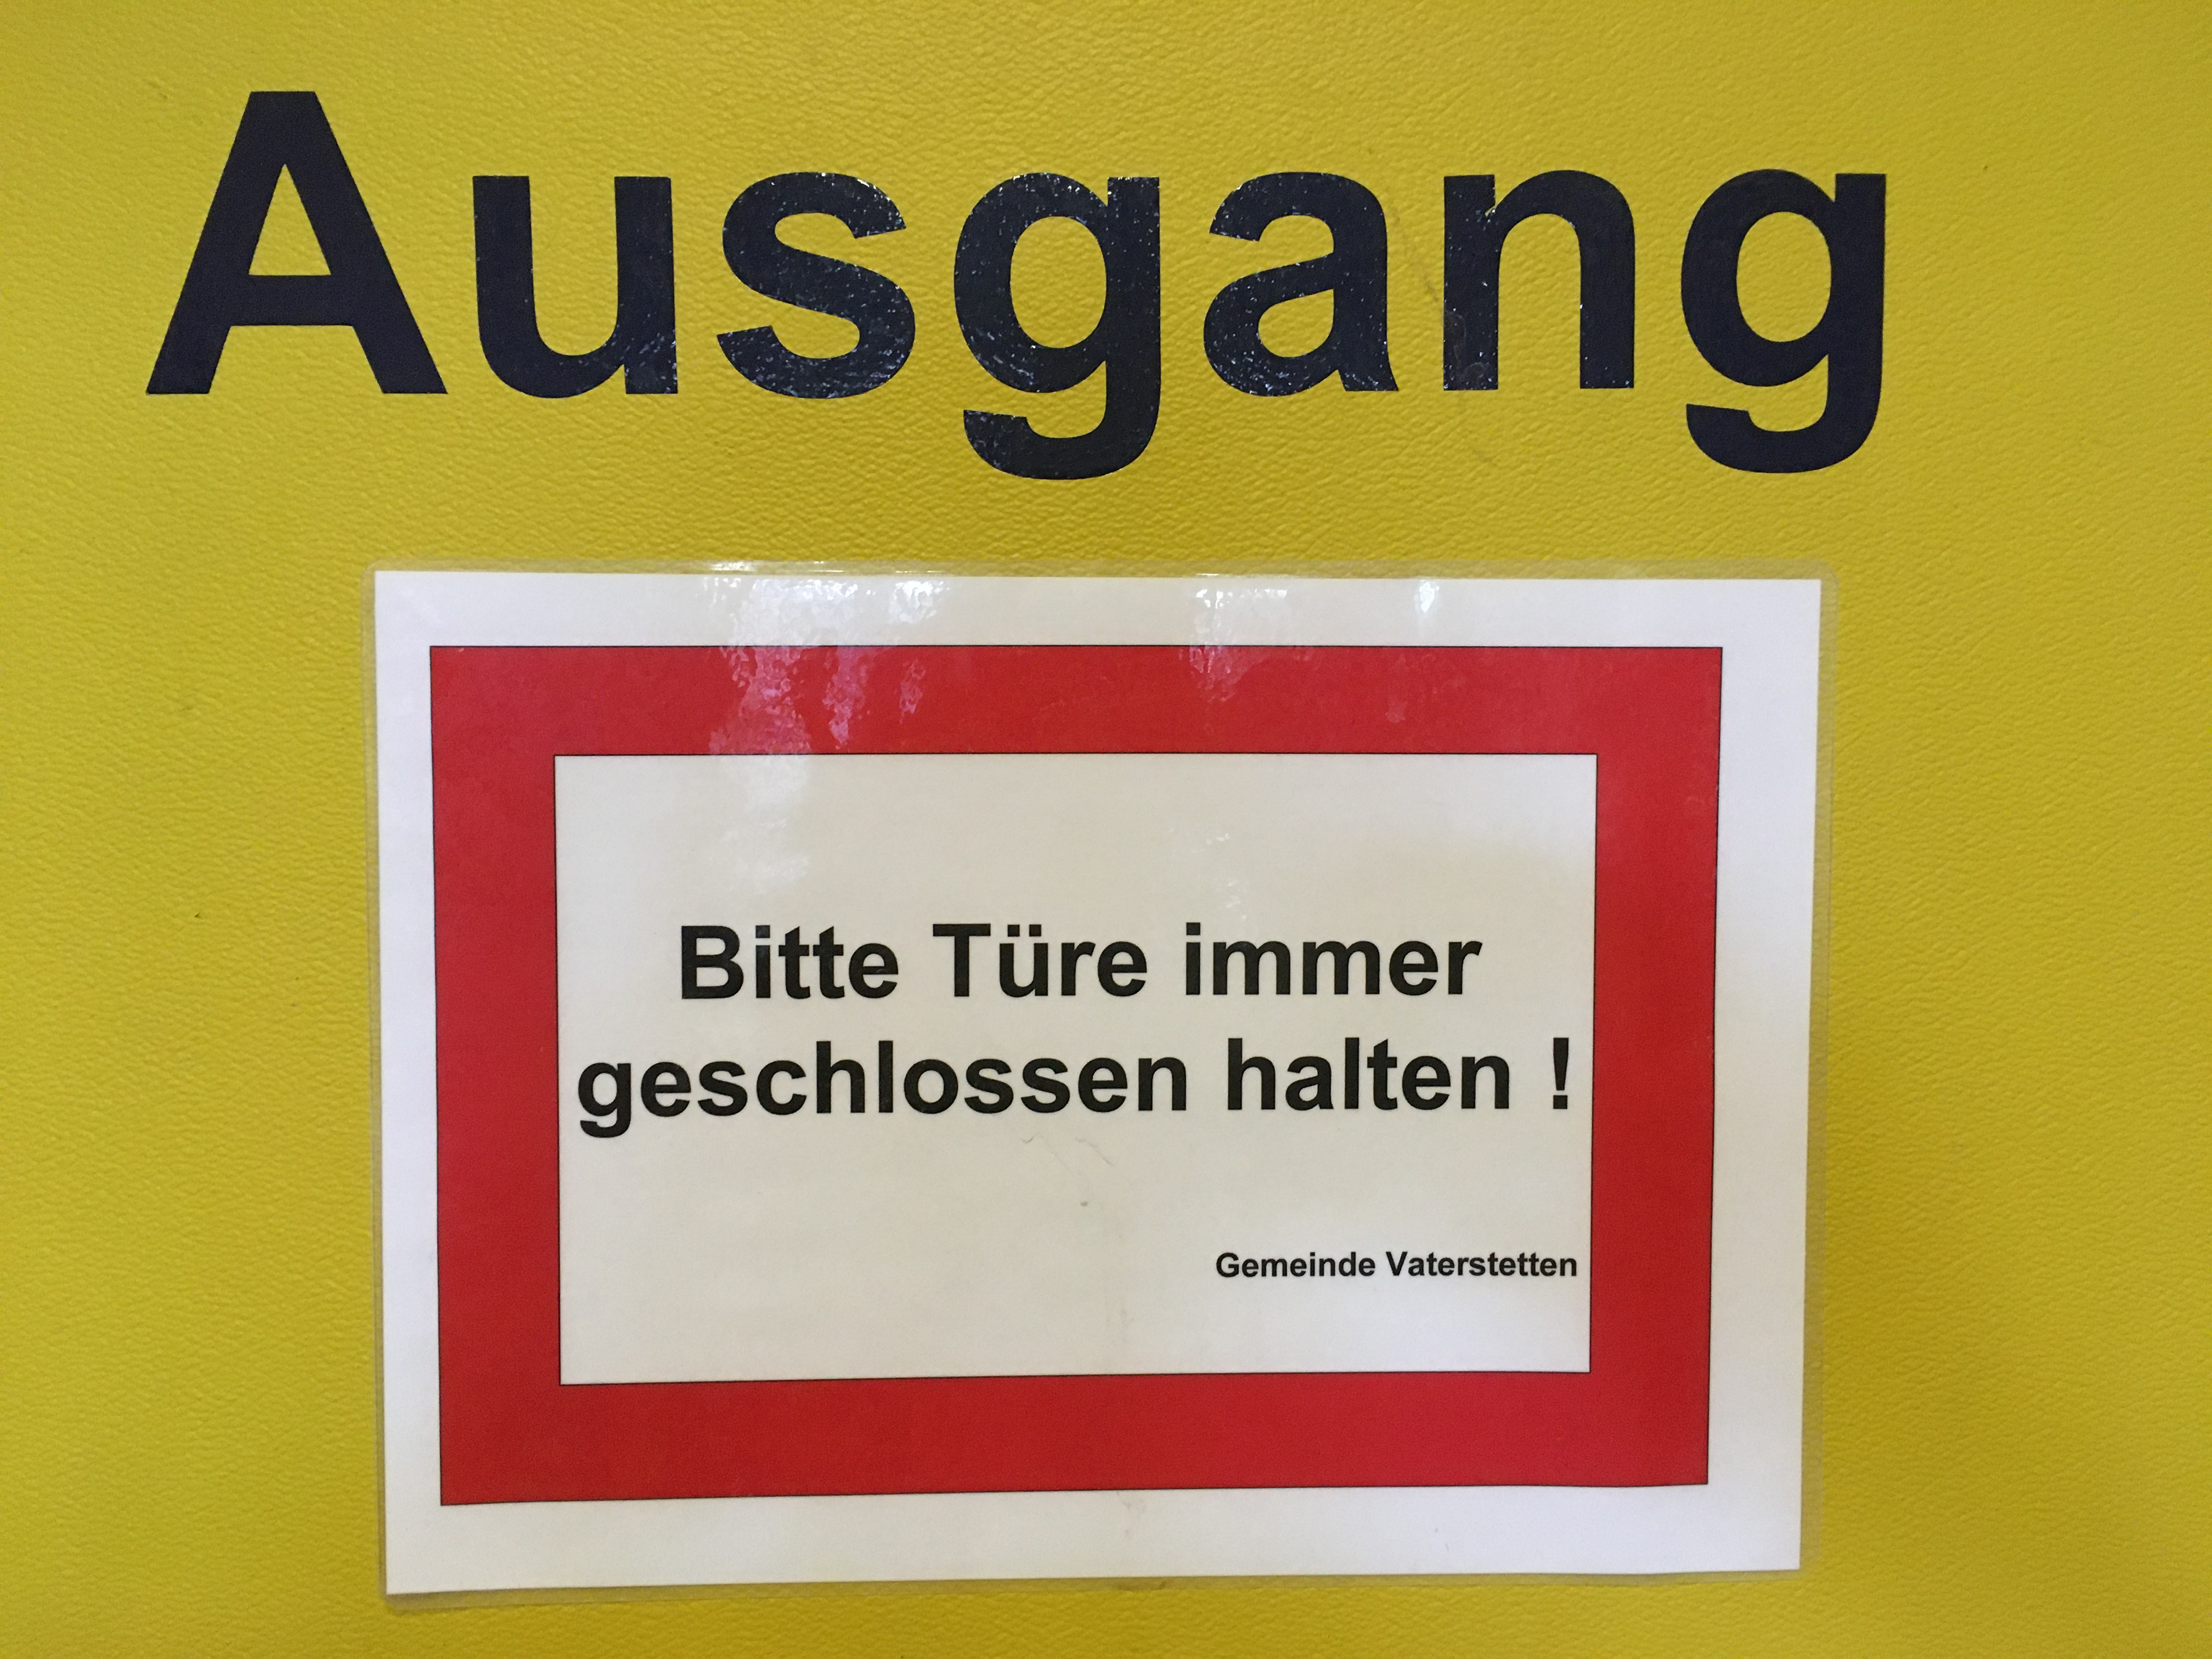
\includegraphics[width=.4\textheight]{graphics/keep_door_closed}
    };

  \end{tikzpicture}

\end{frame}



%%%%%%%%%%%%
% AI Does Not Exist
%%%%%%%%%%%%
\begin{frame}[c]{What is AI?}
  \begin{center}
  \huge Artificial Intelligence Does Not Exist
  \end{center}
  \end{frame}

\begin{frame}{What is AI?}
\framesubtitle{Artificial Intelligence does not exist, yet ...}
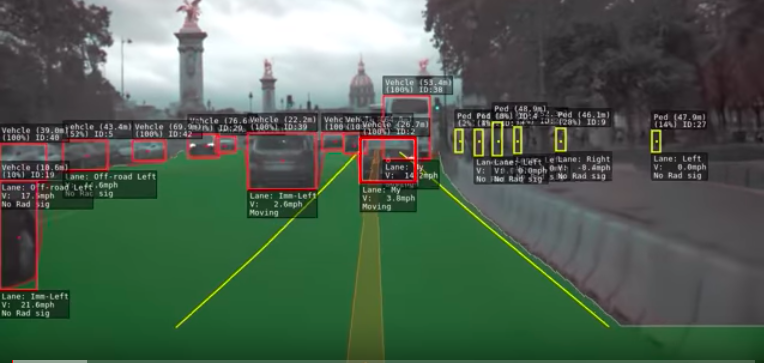
\includegraphics[width=\textwidth]{graphics/tesla_paris}

Source: \href{https://www.youtube.com/watch?v=_1MHGUC_BzQs}{YouTube: greentheonly, Paris streets in the eyes of Tesla Autopilot}
\end{frame}

\begin{frame}{What is AI?}
\framesubtitle{Artificial Intelligence does not exist, yet ...}
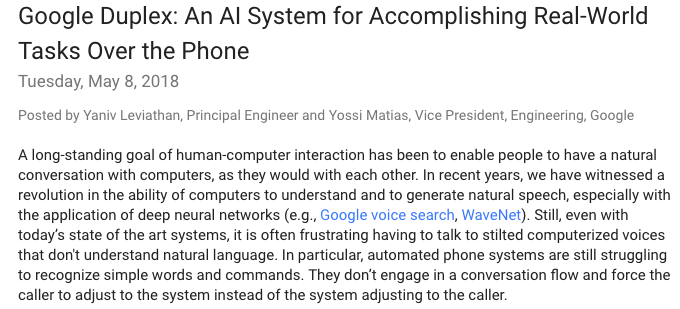
\includegraphics[width=\textwidth]{graphics/google_duplex}

Source: \href{https://ai.googleblog.com/2018/05/duplex-ai-system-for-natural-conversation.html}{Google AI Blog}
\end{frame}

\begin{frame}{What is AI?}
  \framesubtitle{Artificial Intelligence does not exist, yet ...}
  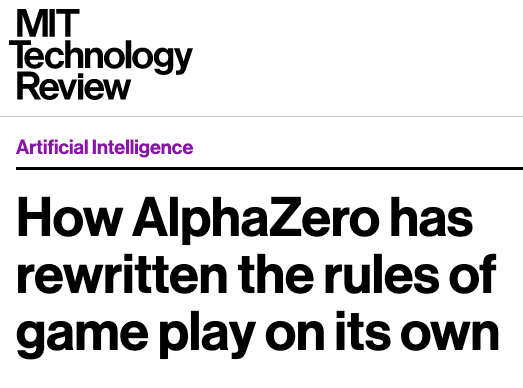
\includegraphics[width=0.8\textwidth]{graphics/alpha_go}

  Source: \href{https://www.technologyreview.com/s/612923/how-alphazero-has-rewritten-the-rules-of-gameplay-on-its-own/}{MIT Technology Review}
\end{frame}

\begin{frame}{AI and Risk}
  \framesubtitle{AI struggles with Context}
  The scientist named the population, after their distinctive horn, Ovid’s Unicorn. These four-horned, silver-white unicorns were previously unknown to science.\newline

  Source: \href{https://www.lesswrong.com/posts/4AHXDwcGab5PhKhHT/humans-who-are-not-concentrating-are-not-general}{https://www.lesswrong.com/posts/4AHXDwcGab5PhKhHT/humans-who-are-not-concentrating-are-not-general}
\end{frame}

\begin{frame}{AI and Risk}
  \frametitle{AI struggles with bias}
  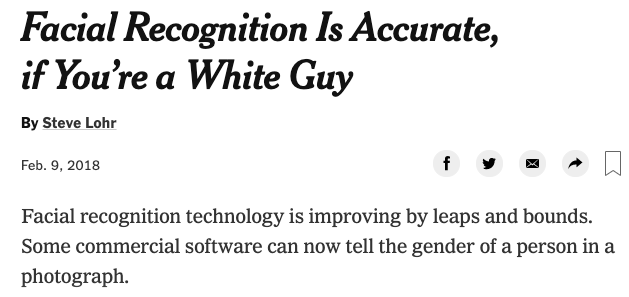
\includegraphics[width=\textwidth]{graphics/facial_bias}

  Source: \href{https://www.nytimes.com/2018/02/09/technology/facial-recognition-race-artificial-intelligence.html}{New York Times}

  See also: \href{https://www.theverge.com/2018/1/12/16882408/google-racist-gorillas-photo-recognition-algorithm-ai}{James Vincent, The Verge, Google 'fixed' its racist algorithm by removing gorillas from its image-labeling tech}
\end{frame}

\begin{frame}{AI and Risk}
  \framesubtitle{AI Struggles With Human Behavior}
  \href{run:graphics/siri_smart_sarcasm.m4a}{Siri Compliments}

  \begin{center}
    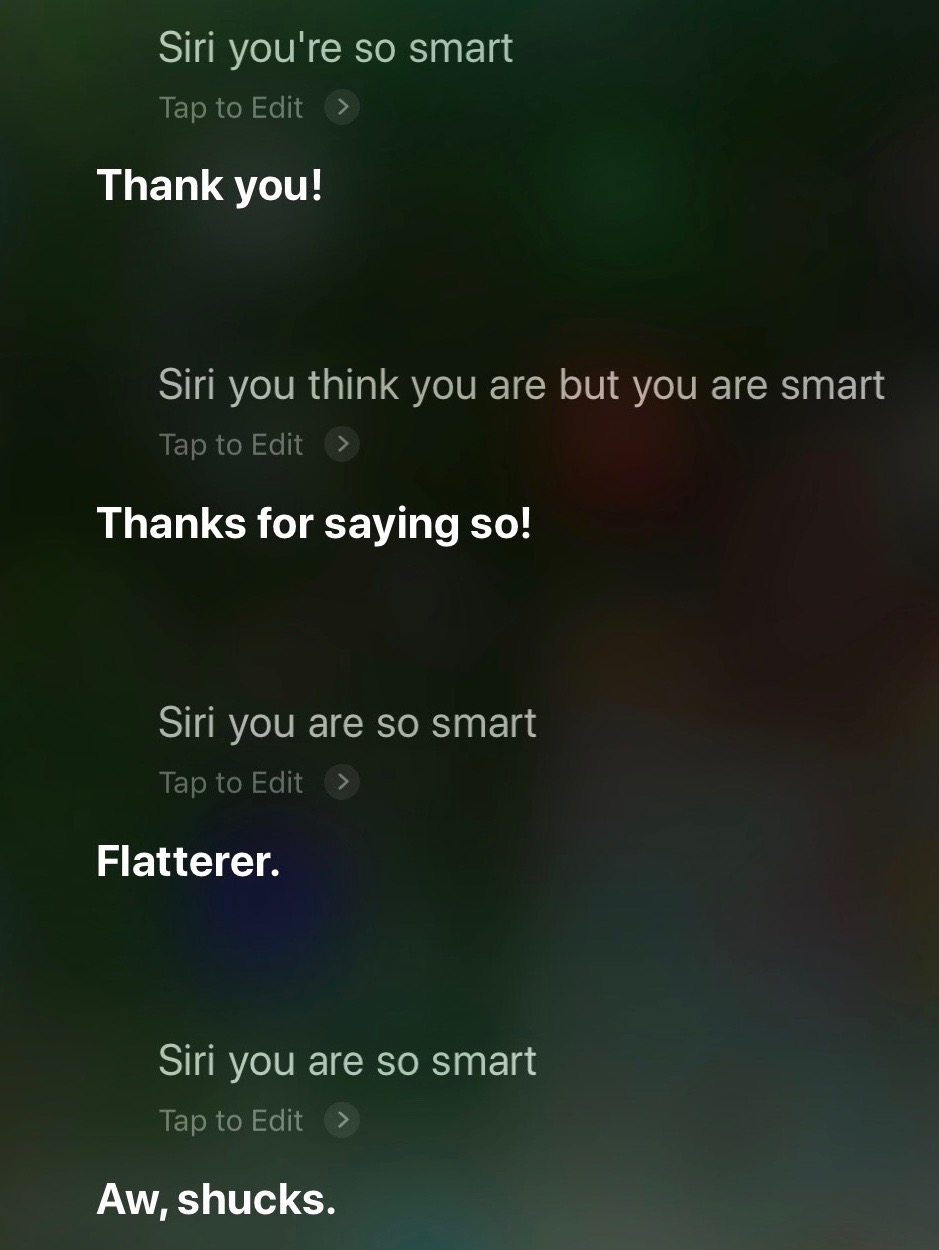
\includegraphics[height=0.7\textheight]{graphics/siri_transcript}
  \end{center}
\end{frame}

\begin{frame}{AI: Where is the crisis?}
  \framesubtitle{Hint, it is not financial, but societal \ldots}
  \begin{quotation}
    AI systems used in education or vocational training, notably for determining access or assigning persons to educational and vocational training institutions or to evaluate persons on tests as part of or as a precondition for their education should be considered high-risk.
  \end{quotation}
  From \href{https://eur-lex.europa.eu/resource.html?uri=cellar:e0649735-a372-11eb-9585-01aa75ed71a1.0001.02/DOC_1&format=PDF}{paragraph 35 of the AI Act}
  \newline
  \href{https://www.fastcompany.com/90342596/schools-are-quietly-turning-to-ai-to-help-pick-who-gets-in-what-could-go-wrong}{FastCompany: AI in admissions, what could go wrong?}
  \newline
  \href{https://www.wired.com/story/algorithm-set-students-grades-altered-futures/}{Wired: The algorithms that keep students out of college}
  \newline
  \href{https://www.theverge.com/2020/8/17/21372045/uk-a-level-results-algorithm-biased-coronavirus-covid-19-pandemic-university-applications}{Verge: UK ditches biased algorithm for university admission}

\end{frame}

\begin{frame}
\frametitle{Workshop topics}
\begin{enumerate}
\item Introduction
\item Discrete geometry for artificial intelligence and risk
\item Correlation and causation
\item Risk and AI in practice
\end{enumerate}
\end{frame}

\begin{frame}
\frametitle{Workshop format}

\begin{itemize}
\item For each topic, lecture + tutorial
\item Emphasis on examples with data produced via python package \href{https://munichpavel.github.io/fake-data-for-learning/}{fake-data-for-learning}
\item Light on non-mathematical definitions, thanks to
\end{itemize}
\centering
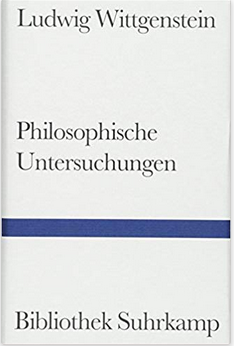
\includegraphics[width=0.3\textheight]{graphics/pi_wittgenstein}
\end{frame}

\end{document}